% !TEX root = ../report.tex

\appendix
\clearpage
\pagenumbering{Roman}
\setcounter{page}{1}

\chapter{Data}\label{app:req}
    \begin{table}[H]
        \centering
        \begin{tabular}{l|l}
            \toprule
            \emph{Variable}        & \emph{Example}   \\ \hline
            "app\_version"   &   0.3  \\ \hline
            "user\_agent"    &   "SOBAZAR 0.3 (iPhone; iPhone OS 6.1.4; Scale/2.00; nb\_NO)"   \\ \hline
            "product\_type"  &   "product"    \\ \hline
            "server\_time\_stamp" &   "2013-10-24T11:33:17.632Z"   \\ \hline
            "dy"    &   24   \\ \hline
            "origin\_ui" &   "storefront"     \\ \hline
            "currency"  &   "kr"     \\ \hline
            "country\_name"  &   "Norway"     \\ \hline
            "price" &   1995     \\ \hline
            "product\_name"  &   "DWS No47"   \\ \hline
            "tag\_name"  &   "NULL"   \\ \hline
            "tag\_id"    &   "NULL"   \\ \hline
            "storefront\_name"   &   "BIK BOK"    \\ \hline
            "event\_id"  &   "product\_purchase\_intended"  \\ \hline
            "age\_target"    &   "Any"    \\ \hline
            "epoch\_day" &   16002    \\ \hline
            "mo"    &   10   \\ \hline
            "yr"    &   2013     \\ \hline
            "product\_id"    &   2298002  \\ \hline
            "event\_location"    &   Geo Location     \\ \hline
            "ipAddress" &   IP  \\ \hline
            "contentDescription"    &   null     \\ \hline
            "sessionId" &   null     \\ \hline
            "contentId" &   null     \\ \hline
            "instKey"   &   "ed4c76251ac47da54299d8c0bce3dca6"   \\ \hline
            "viewer"    &   null     \\ \hline
            "ts"    &   NumberLong("1382614397632")  \\ \hline
            "gender\_target" &   "Female"     \\ \hline
            "client\_time\_stamp" &   "NULL"   \\ \hline
            "login\_type"    &   "NULL"   \\ \hline
            "transaction\_id"    &   "N/A"    \\ \hline
            "service\_id"    &   "SOBAZAR"    \\ \hline
            "platform"  &   "iPhone"     \\ \hline
            "epoch\_week"    &   2286     \\ \hline
            "storefront\_id" &   23002    \\ \hline
            "hr"    &   11   \\ \hline
            "tag\_position"  &   "NULL"   \\ \hline
            "time\_stamp"    &   "2013-10-24T13:33+0200"  \\ \hline
            "retailer\_brand"    &   13001    \\ \hline
            "storefront\_position"   &   2    \\ \hline
            "user\_id"   &   1342189870   \\ \hline
            "country\_id"    &   194001   \\ \hline
            "server\_environment"    &   "prod" \\
            \bottomrule
        \caption[Complete List of Event Metadata]{Table of the complete list of event metadata stored when an event is triggered}
        \label{table:completeEventData}
        \end{tabular}
    \end{table}
    \marginpar{TODO: Add an explanation to each row, and maybe remove example?}

    \begin{table}[H]
        \centering
        \begin{tabular}{l|l}
            \toprule
            \emph{Event Name}     & \emph{Explanation}   \\ \hline
            "product\_wanted"            & - \\ \hline
            "product\_detail\_clicked"    & - \\ \hline
            "storefront\_clicked"        & - \\ \hline
            "activity\_clicked"          & - \\ \hline
            "around\_me\_clicked"         & - \\ \hline
            "user\_logged\_in"            & - \\ \hline
            "featured\_storefront\_clicked"   & - \\ \hline
            "friend\_invited"    & - \\ \hline
            "app\_started"   & - \\ \hline
            "stores\_map\_clicked"    & - \\ \hline
            "product\_purchase\_intended" & - \\ \hline
            "store\_clicked" & - \\ \hline
            "featured\_collection\_clicked" & - \\
            \bottomrule
        \caption[List of Different Events]{Table of the different events that can be triggered by the user and an explanation}
        \label{table:events}
        \end{tabular}
    \end{table}
    \marginpar{TODO: Add all the different event types}


    \begin{figure}[H]
        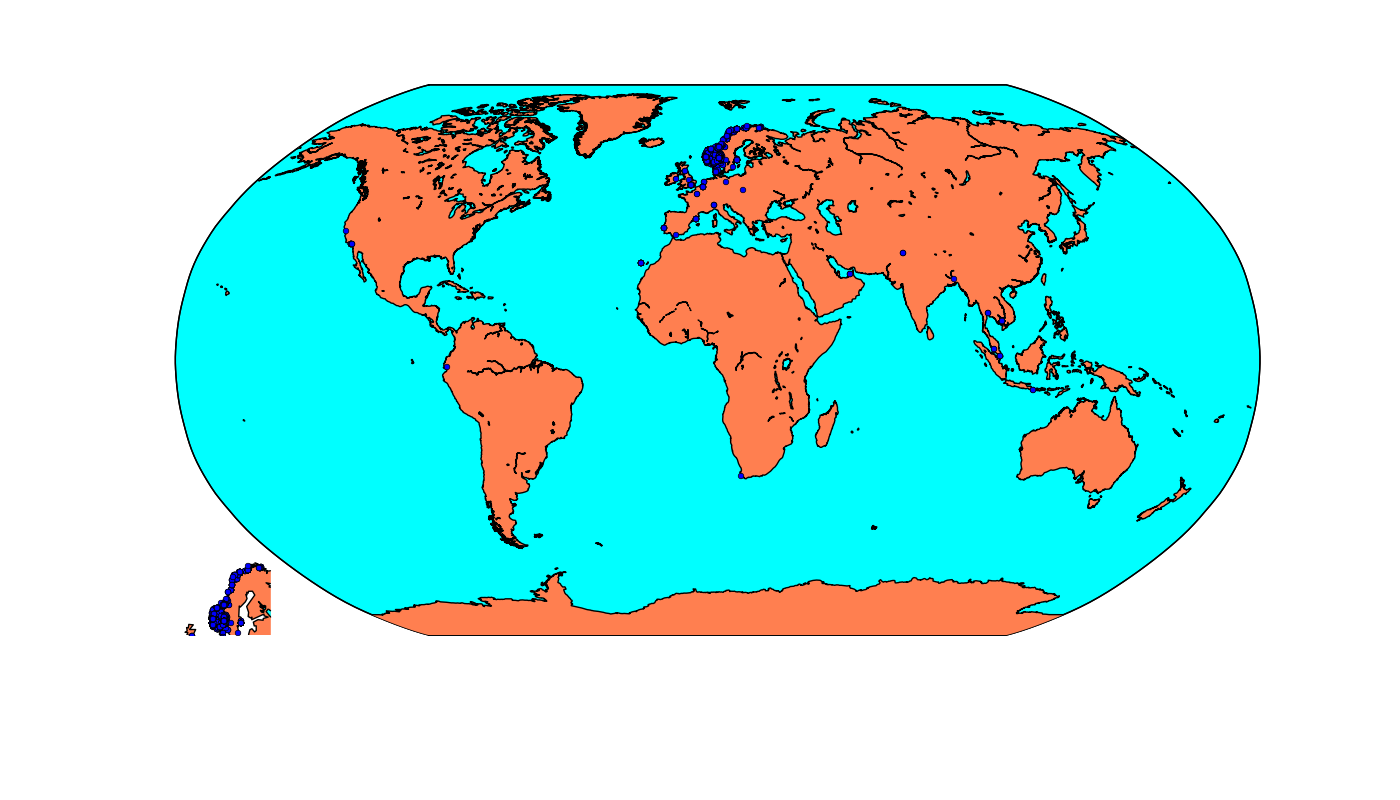
\includegraphics[width=5in]{image/simpleGeoPlotworld.png}
        \centering
        \caption[Event location mapped on the world]{This figure shows the location of the events from all over the world.
        For a cropped version with focus on Norway and the surrounding countries, refer to~\ref{figure:croppedGeoplot}}
    \end{figure}

    \begin{figure}[H]
        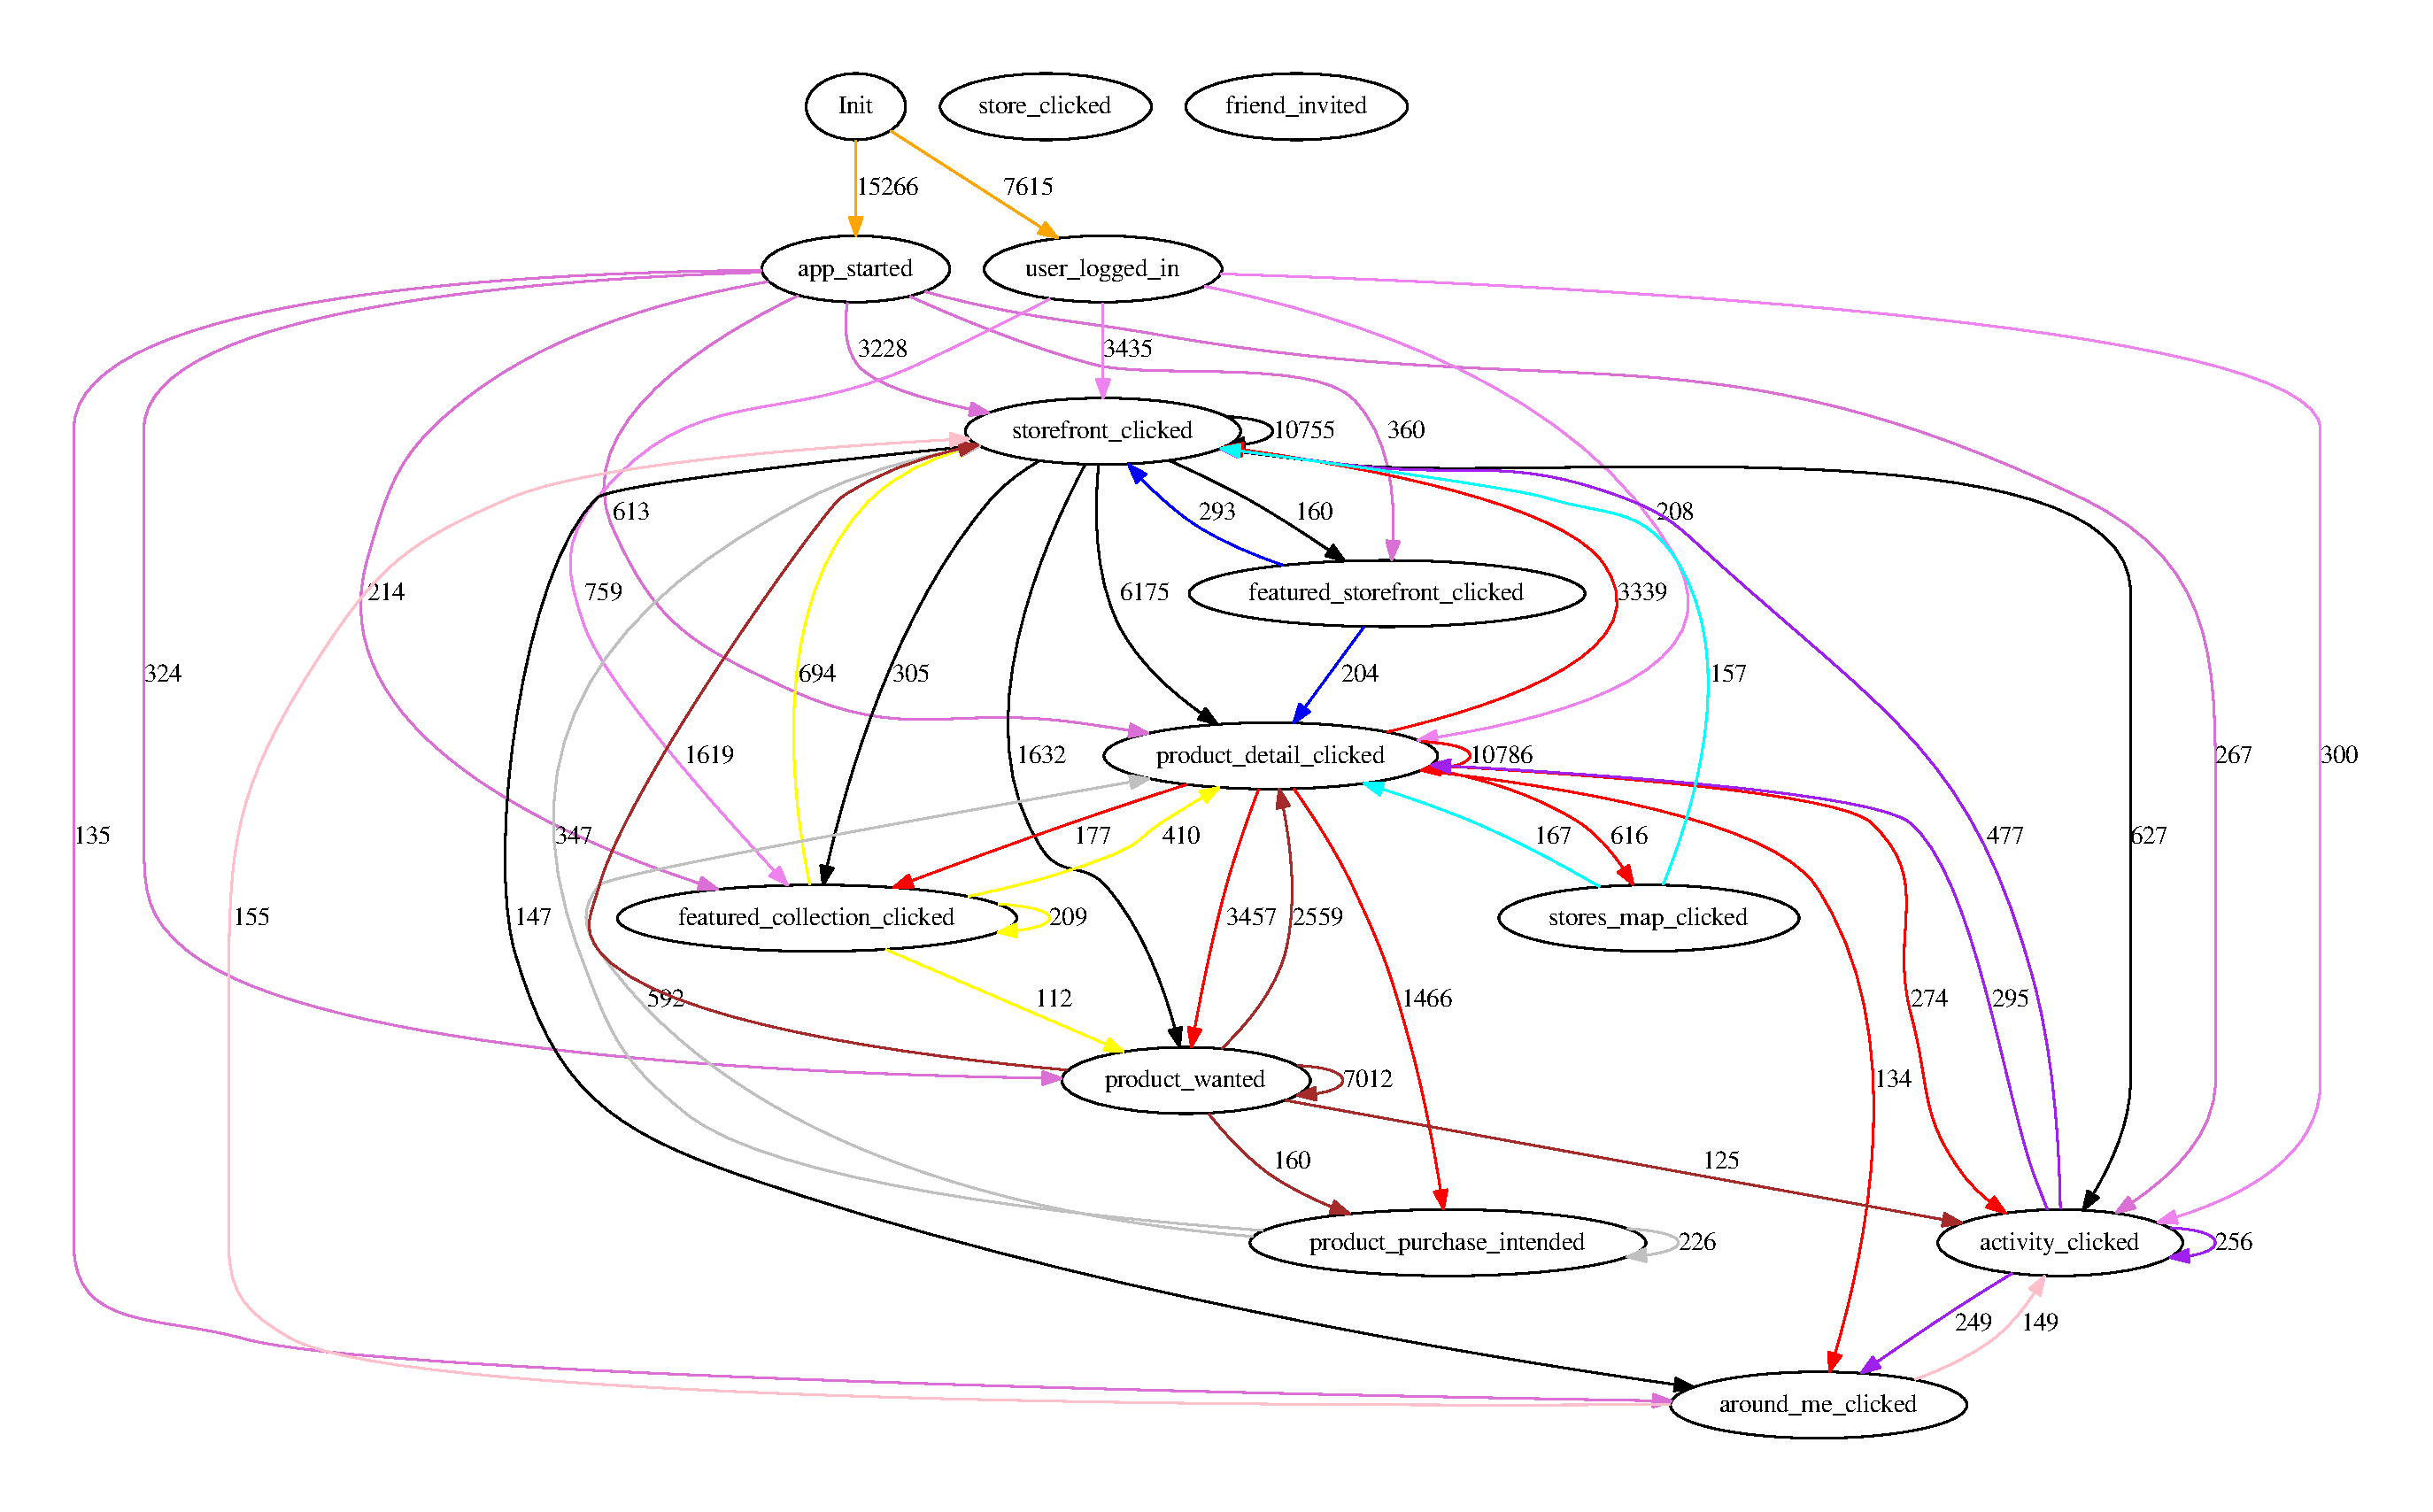
\includegraphics[width=5in]{image/statesInteractionFalse-gvfile.pdf}
        \centering
        \caption[States in session and how they interact]{The different states of the system and how they interact with each other.}
        \label{figure:statesInteractions}
    \end{figure}

\chapter{Requirements}\label{app:req}

\section{Functional Requirements}

\section{Non Functional Requirements}

\chapter{Design}\label{app:des}

\chapter{Implementation}\label{app:impl}
\section{Implemented Functional Requirements}
\begin{enumerate}[label=\bfseries FR \arabic*:]
  \item {\color{ForestGreen}Blablaba}
  \item {\color{RedOrange}\st{Blablaba}}
\end{enumerate}

\section{Implemented Non Functional Requirements}
\begin{enumerate}[label=\bfseries NFR \arabic*:]
  \item {\color{ForestGreen}Blablaba}
  \item {\color{RedOrange}\st{Blablaba}}
\end{enumerate}

